\documentclass[11pt,a4paper]{article}
\usepackage[margin=2.3cm]{geometry}
\usepackage[T1]{fontenc}
\usepackage{mathpazo}
\renewcommand{\ttdefault}{txtt}
\usepackage{microtype}
\usepackage{amsmath,amssymb}
\usepackage{graphicx}
\usepackage{booktabs}
\usepackage{float}
\usepackage[font=small,labelfont=bf]{caption}
\usepackage{subcaption}
\usepackage{xcolor}
\usepackage{enumitem}
\usepackage{fancyhdr}
\usepackage{listings}
\usepackage{tikz}
\usetikzlibrary{positioning,arrows.meta,shapes.misc}
\usepackage[ruled,linesnumbered,vlined]{algorithm2e}
\usepackage[colorlinks=true,linkcolor=black,citecolor=black,urlcolor=blue!50!black]{hyperref}

\definecolor{licit}{HTML}{2a78d6}
\definecolor{illicit}{HTML}{eb6834}
\definecolor{codebg}{HTML}{f5f5f4}
\lstset{basicstyle=\ttfamily\footnotesize,backgroundcolor=\color{codebg},frame=single,rulecolor=\color{black!25},
  columns=fullflexible,keepspaces=true,showstringspaces=false,commentstyle=\itshape\color{black!55},
  keywordstyle=\bfseries,language=Python,aboveskip=6pt,belowskip=6pt}
\setlist{itemsep=2pt,topsep=4pt}
\pagestyle{fancy}\fancyhf{}
\fancyhead[R]{\small GCN: Illicit Transaction Detection on the Elliptic Bitcoin Network}
\fancyfoot[C]{\thepage}
\renewcommand{\headrulewidth}{0pt}
\newcommand{\Ahat}{\hat{A}}

\title{\vspace{-1.2cm}\textbf{GCN: Illicit Transaction Detection on the\\ Elliptic Bitcoin Network}\\[4pt]
\large Anti-money-laundering as node classification with a 2-layer Graph Convolutional Network}
\author{\textbf{[Your name]} \\ \textcolor{red}{[roll no.]}}
\date{}

\begin{document}
\maketitle
\thispagestyle{fancy}

\begin{abstract}
\noindent We apply the Graph Convolutional Network (GCN) of Kipf and Welling \cite{kipf} to a real anti-money-laundering task:
classifying the 203,769 Bitcoin transactions of the Elliptic dataset \cite{weber} as \emph{licit} or \emph{illicit}. The propagation
rule is implemented from scratch as sparse matrix products, not with a library layer. The task is harder than citation or co-purchase
benchmarks: only 9.8\% of labelled transactions are illicit, the graph is split into 49 time steps and the model is tested on
\emph{future} ones, and strong tabular baselines exist. Trained on time steps 1--34 and tested on 35--49, the two-layer GCN reaches an
illicit F1 of \textbf{0.560 $\pm$ 0.034} over 5 seeds (0.572 for seed 42). Compared with the same network without the graph, it is far
more precise (0.79 versus 0.56) and ranks illicit transactions much better (average precision 0.60 versus 0.44), but its F1 is only
slightly higher, and with local features only the graph does not help F1 at all. A Random Forest remains the strongest model (0.810), as in the
original benchmark. We analyse the training behaviour, the effect of class imbalance, and over-smoothing in trained models of increasing
depth. We also show that every model fails after a dark-market shutdown at time step 43, which makes concept drift the main open problem.
\end{abstract}

%=====================================================================
\section{The Elliptic Bitcoin Dataset}
%=====================================================================
Bitcoin is pseudonymous: every transaction is public, but the people behind it are not. This makes it attractive for
ransomware, scams, darknet markets and Ponzi schemes, and it gives financial institutions an \emph{anti-money-laundering}
(AML) problem: which transactions should be flagged? The \textbf{Elliptic dataset} \cite{weber}, released by the blockchain
analytics company Elliptic together with MIT-IBM Watson AI Lab, is the largest public labelled transaction graph for this task.
It is a graph in which
\begin{itemize}
  \item each \textbf{node} is a Bitcoin transaction (203,769 in total);
  \item each \textbf{edge} is a flow of bitcoin: an output of one transaction is spent as an input of the next
        (234,355 directed edges);
  \item each node has a \textbf{feature vector} of 165 anonymised values: 93 \emph{local} features of the transaction itself
        (number of inputs/outputs, fee, output volume, \dots) and 72 \emph{aggregated} features that summarise its one-hop
        neighbours (maxima, minima, standard deviations, correlations);
  \item each node carries a \textbf{time step} from 1 to 49 (roughly two weeks apart) and a \textbf{label}: illicit
        (4,545), licit (42,019) or unknown (157,205).
\end{itemize}
Figure~\ref{fig:ego} shows a real piece of the graph, the \emph{Wallet $\rightarrow$ Tx $\rightarrow$ Tx $\rightarrow$ Tx} chain
of the problem statement: about twenty illicit transactions, including the highlighted one, all send funds into the same
unlabelled transaction, a typical ``fan-in'' pattern for collecting proceeds. Such a pattern is invisible to a model that looks at one transaction at a time,
and it is exactly what a GCN can use.

\begin{figure}[H]
  \centering
  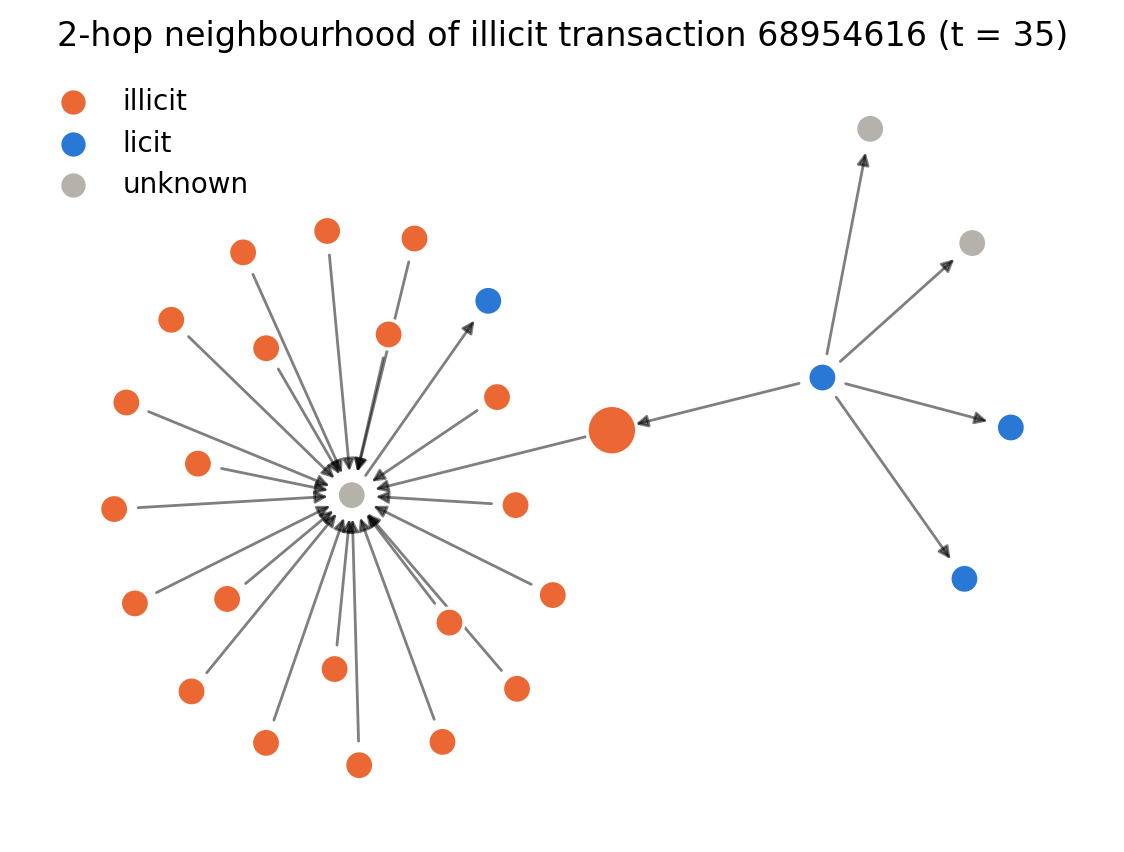
\includegraphics[width=0.62\linewidth]{figures/ego_graph.png}
  \caption{Two-hop neighbourhood of an illicit test transaction (large node). Arrows follow the flow of bitcoin.}
  \label{fig:ego}
\end{figure}

\noindent Three properties set Elliptic apart from Cora or Amazon Photo (Table~\ref{tab:data}):
\begin{itemize}
  \item \textbf{Imbalance.} Only 9.8\% of labelled nodes are illicit, and 77\% of nodes have no label at all.
        On the test period a model that always answers ``licit'' is 93.5\% accurate yet catches no criminal,
        so accuracy is useless as a metric; we use the \emph{illicit F1 score}.
  \item \textbf{Time.} No edge connects two time steps, so the graph is made of 49 separate transaction graphs and has exactly
        49 connected components, one per time step. We follow the \textbf{temporal split} of Weber et al.: train on time steps
        1--34 and test on 35--49. Test transactions therefore sit in graphs the model has never seen: the GCN must
        generalise \emph{inductively} to new graphs, not only to new nodes of a known graph.
  \item \textbf{Sparsity and homophily.} The average degree is only 2.30 (median 2, max 473). Among edges whose two ends are
        labelled, 95.4\% join transactions of the same class, and a labelled neighbour of an illicit transaction is illicit
        54.1\% of the time, against a base rate of 9.8\% (and 2.4\% for neighbours of licit transactions).
        The graph therefore carries a strong signal.
\end{itemize}

\begin{table}[H]
\centering\small
\begin{tabular}{ll}
\toprule
Nodes / features / classes & 203,769 / 165 / 2 (+ unknown) \\
Edges & 234,355 directed (treated as undirected for the GCN) \\
Labels & 4,545 illicit / 42,019 licit / 157,205 unknown \\
Time steps / connected components & 49 / 49 \\
Train (time steps 1--34) & 29,894 labelled, 3,462 illicit (11.6\%) \\
Test (time steps 35--49) & 16,670 labelled, 1,083 illicit (6.5\%) \\
Average degree & 2.30 \\
\bottomrule
\end{tabular}
\caption{The Elliptic dataset as loaded in the notebook.}
\label{tab:data}
\end{table}

\begin{figure}[H]
  \centering
  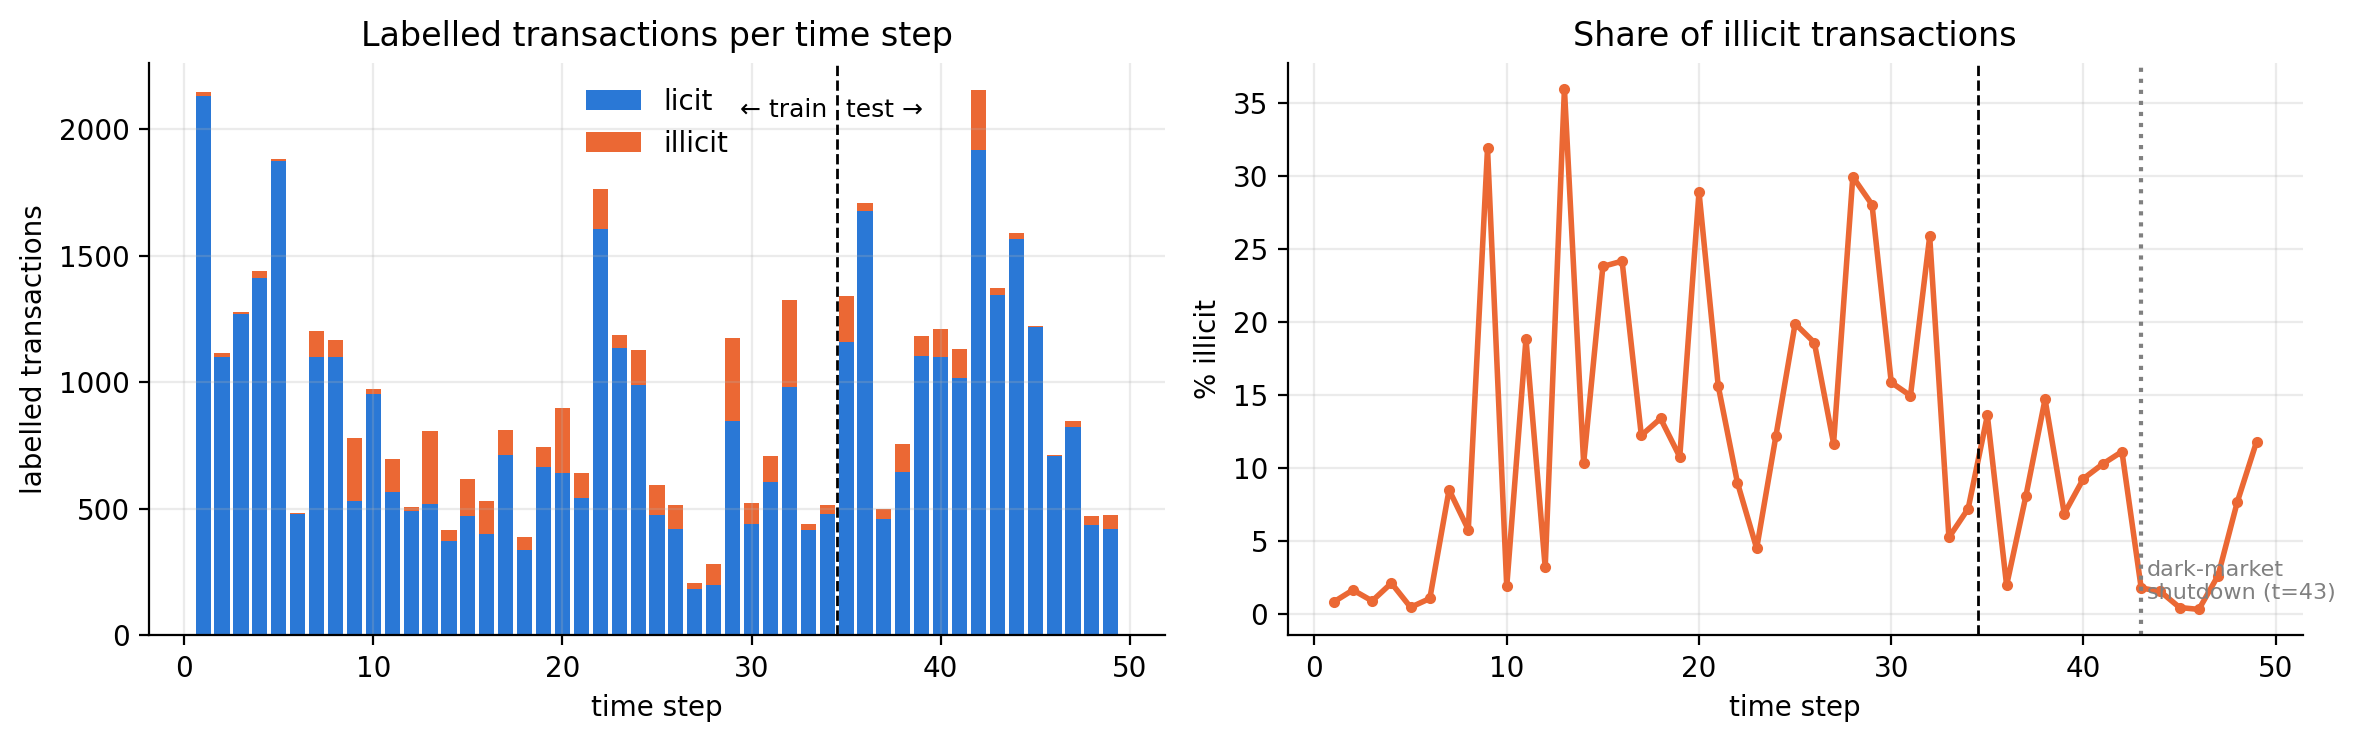
\includegraphics[width=\linewidth]{figures/dataset_timesteps.png}
  \caption{Labelled transactions per time step (left) and the share that is illicit (right). The dashed line is the
  train/test boundary; the dotted line marks the dark-market shutdown reported by Weber et al.}
  \label{fig:timesteps}
\end{figure}

%=====================================================================
\section{Introduction: What, Why and How of a GCN}
%=====================================================================
\subsection{What is a GCN?}
A \textbf{Graph Convolutional Network} is a neural network that works directly on graph-structured data. An image has a
fixed grid, so a convolution can slide one filter over it; a node in a graph has a variable number of unordered neighbours,
so ordinary convolution does not apply. A GCN replaces the sliding filter by \emph{neighbourhood aggregation}: in every layer, each
node's representation is recomputed from its own features and those of its neighbours, with the same weights for all nodes.
After $k$ layers a node has seen information from up to $k$ hops away.

\subsection{Why use a GCN for fraud detection?}
\begin{itemize}
  \item \textbf{Crime leaves a structural trace.} Illicit funds are split, merged and relayed through chains of transactions.
        Whether a transaction is suspicious depends on where its money came from and where it goes, not only on its own amount or fee.
  \item \textbf{Few labels, many nodes.} Only 23\% of transactions are labelled. The unlabelled ones still pass messages, so a label
        near them informs their neighbours.
  \item \textbf{Efficiency.} A layer touches only existing edges, so its cost grows with the number of edges; the Elliptic graph with
        about 670 thousand non-zeros is processed in well under a second on a laptop CPU.
  \item \textbf{No node ordering.} Relabelling the transactions only permutes the rows of the output.
\end{itemize}

\subsection{How does it work?}
Let the graph have $N$ nodes, adjacency matrix $A\in\mathbb{R}^{N\times N}$ and feature matrix $X\in\mathbb{R}^{N\times F}$.
We first add self-loops so that a node keeps its own information, then normalise by degree:
\begin{equation}
  \Ahat = \tilde D^{-1/2}\,\tilde A\,\tilde D^{-1/2},\qquad \tilde A = A + I_N,\qquad \tilde D_{ii} = \sum_j \tilde A_{ij}.
  \label{eq:ahat}
\end{equation}
One GCN layer is
\begin{equation}
  H^{(l+1)} = \sigma\!\left(\Ahat\,H^{(l)}\,W^{(l)}\right),\qquad H^{(0)} = X,
  \label{eq:layer}
\end{equation}
where $W^{(l)}$ is a weight matrix shared by all nodes and $\sigma$ is a non-linearity (ReLU). The product $H W$ transforms every
node's features in the same way, and multiplying by $\Ahat$ aggregates them over the neighbourhood. For a single node $v$,
\begin{equation}
  h_v^{(l+1)} = \sigma\Big(\sum_{u\in\mathcal N(v)\cup\{v\}} \frac{1}{\sqrt{\tilde d_u\,\tilde d_v}}\; h_u^{(l)}W^{(l)}\Big),
  \label{eq:node}
\end{equation}
a degree-weighted average over the node and its neighbours. The symmetric weights matter on Elliptic: some transactions
have hundreds of inputs or outputs (maximum degree 473), and without the $1/\sqrt{\tilde d_u \tilde d_v}$ factor
such hubs would dominate their neighbours' representations.

\subsection{Where the propagation rule comes from}
The layer rule is a simplified \emph{spectral} graph convolution \cite{kipf}.
\textbf{(1) Laplacian.} With degree matrix $D$, the normalised Laplacian is $L = I - D^{-1/2} A D^{-1/2}$. For a signal $f$ on the
nodes, $f^\top L f = \tfrac12\sum_{i,j} A_{ij}\big(f_i/\sqrt{d_i} - f_j/\sqrt{d_j}\big)^2$, so $L$ measures how much $f$ varies
across edges. \textbf{(2) Graph Fourier basis.} $L$ is symmetric positive semi-definite, $L = U\Lambda U^\top$; eigenvectors with small
eigenvalues are smooth over the graph, those with large eigenvalues oscillate. A spectral filter is
$g_\theta \star f = U g_\theta(\Lambda) U^\top f$. \textbf{(3) Polynomial filters.} Computing $U$ costs $O(N^3)$, impossible for
$N\approx 2\times10^5$. Approximating $g_\theta$ by a polynomial of degree $K$ in $L$ removes the eigendecomposition and makes the filter
$K$-hop local, because $(L^K)_{ij}=0$ for nodes more than $K$ hops apart. \textbf{(4) First order.} Kipf and Welling keep $K=1$,
approximate the largest eigenvalue by 2 and tie the two coefficients, giving $g_\theta\star f \approx \theta\,(I + D^{-1/2}AD^{-1/2})f$.
\textbf{(5) Renormalisation trick.} $I + D^{-1/2}AD^{-1/2}$ has eigenvalues in $[0,2]$, so stacking it makes activations explode or
vanish. Replacing it by $\Ahat$ of Eq.~(\ref{eq:ahat}), whose eigenvalues lie in $(-1,1]$, and generalising $\theta$ to a
matrix $W$, gives Eq.~(\ref{eq:layer}).

%=====================================================================
\section{Working Mechanism of Our GCN}
%=====================================================================
\subsection{Task}
Given the transaction graph of Section~1, predict for every labelled transaction in time steps 35--49 whether it is illicit, using
its 165 features, the graph structure and the labels of time steps 1--34 only.

\subsection{The model}
Stacking two layers of Eq.~(\ref{eq:layer}) with a softmax output gives
\begin{equation}
  Z = \mathrm{softmax}\!\Big(\Ahat\;\mathrm{ReLU}\big(\Ahat\,X\,W^{(0)} + b^{(0)}\big)\,W^{(1)} + b^{(1)}\Big),
  \label{eq:model}
\end{equation}
with $X\in\mathbb{R}^{203769\times165}$, $W^{(0)}\in\mathbb{R}^{165\times100}$, $W^{(1)}\in\mathbb{R}^{100\times2}$, and $Z_{i,1}$ the
predicted probability that transaction $i$ is illicit. We flag transaction $i$ when $Z_{i,1}\ge 0.5$.

We also study two variants built from the same code. The \textbf{MLP} replaces $\Ahat$ by the identity $I$ and so sees only each
transaction's own features; comparing it with the GCN isolates the contribution of the graph. The \textbf{Skip-GCN} of Weber et al.\
adds a linear path from the input to the output,
\begin{equation}
  Z = \mathrm{softmax}\!\Big(\Ahat\;\mathrm{ReLU}\big(\Ahat X W^{(0)}+b^{(0)}\big)W^{(1)} + b^{(1)} + X W_{\text{skip}}\Big),
  \label{eq:skip}
\end{equation}
so that a transaction's own evidence reaches the output without being averaged with its neighbours'.

\subsection{Loss for an imbalanced problem}
With about one illicit transaction in ten, an unweighted cross-entropy is minimised quite well by predicting ``licit'' for almost
everything. Following \cite{weber}, we use a \textbf{weighted cross-entropy} with $w_{\text{licit}}=0.3$ and $w_{\text{illicit}}=0.7$
over the labelled training set $\mathcal Y_L$:
\begin{equation}
  \mathcal L = -\frac{1}{\sum_{i\in\mathcal Y_L} w_{y_i}} \sum_{i\in\mathcal Y_L} w_{y_i}\,\ln Z_{i,y_i}.
  \label{eq:loss}
\end{equation}
The loss uses only the 29,894 labelled training transactions, but gradients flow through $\Ahat$, so unlabelled transactions shape
the hidden representations of their labelled neighbours.

\subsection{Metrics}
With $TP$, $FP$, $FN$ counted for the illicit class, \emph{precision} $=TP/(TP+FP)$ is the share of flagged transactions that really
are illicit (the cost of false alarms for an investigator), \emph{recall} $=TP/(TP+FN)$ is the share of illicit transactions that are
caught, and the \textbf{illicit F1} $= 2PR/(P+R)$ is the benchmark's headline metric. We also report micro-F1 (equal to accuracy) and
the average precision (AP, the area under the precision--recall curve), which does not depend on the 0.5 threshold.

\subsection{Algorithm}
\begin{algorithm}[H]
\small
\caption{Training and evaluation, as implemented in the notebook}
\KwIn{graph $(A,X)$, labels $Y$, masks $\mathcal M_{\text{train}}$ (t 1--34), $\mathcal M_{\text{test}}$ (t 35--49)}
Standardise $X$ with the mean and std of time steps 1--34; build $\Ahat$ once (sparse)\;
Compute $P \leftarrow \Ahat X$ once \tcp*{$\Ahat$ and $X$ are fixed}
Initialise $W^{(0)}, W^{(1)}$ (Glorot), biases $\leftarrow 0$\;
\For{epoch $=1$ \KwTo $200$}{
  $Z \leftarrow \Ahat\,\mathrm{ReLU}(P W^{(0)} + b^{(0)})\,W^{(1)} + b^{(1)}$ over the \emph{whole} graph\;
  $\mathcal L \leftarrow$ weighted cross-entropy (Eq.~\ref{eq:loss}) on $\mathcal M_{\text{train}}$ only\;
  back-propagate and take one Adam step\;
  every 10 epochs: log loss and train/test illicit F1 (for plotting only)\;
}
\KwOut{illicit precision, recall, F1 and AP on $\mathcal M_{\text{test}}$ after the final epoch}
\end{algorithm}
\noindent We have no validation period to spare (time steps are few and the test period must stay in the future), so we do
\emph{not} select epochs or hyperparameters on the test set: we fix standard values in advance and report the last epoch.

%=====================================================================
\section{Model Architecture and Implementation}
%=====================================================================
\begin{figure}[H]
\centering
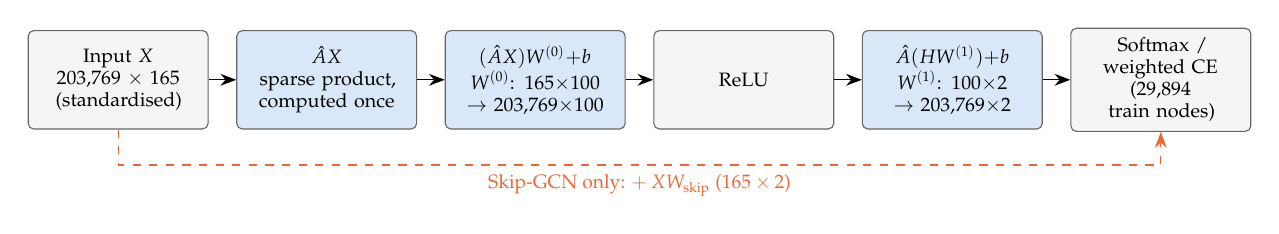
\begin{tikzpicture}[
  box/.style={draw=black!60, rounded corners=2pt, align=center, font=\scriptsize, minimum height=1.25cm, text width=2.05cm, fill=#1},
  box/.default=black!4, >={Stealth[length=2mm]}]
\node[box] (x) {Input $X$\\203,769 $\times$ 165\\(standardised)};
\node[box=licit!18, right=0.35cm of x] (ax) {$\Ahat X$\\sparse product,\\computed once};
\node[box=licit!18, right=0.35cm of ax] (l1) {$(\Ahat X)W^{(0)}{+}b$\\$W^{(0)}$: 165$\times$100\\$\to$ 203,769$\times$100};
\node[box, right=0.35cm of l1] (relu) {ReLU};
\node[box=licit!18, right=0.35cm of relu] (l2) {$\Ahat(HW^{(1)}){+}b$\\$W^{(1)}$: 100$\times$2\\$\to$ 203,769$\times$2};
\node[box, right=0.35cm of l2] (out) {Softmax /\\weighted CE\\(29,894 train nodes)};
\foreach \a/\b in {x/ax, ax/l1, l1/relu, relu/l2, l2/out} \draw[->] (\a) -- (\b);
\draw[->, dashed, illicit] (x.south) -- ++(0,-0.45) -| node[pos=0.25, below, font=\scriptsize] {Skip-GCN only: $+\,XW_{\text{skip}}$ ($165\times2$)} (out.south);
\end{tikzpicture}
\caption{Forward pass of the implemented network with tensor shapes. $\Ahat$ (sparse, fixed, 672,479 non-zeros) is used in both
graph convolutions; only the $W$s and biases are learned.}
\label{fig:arch}
\end{figure}

\noindent The notebook uses plain \textbf{PyTorch}. PyTorch Geometric \cite{pyg} appears only as an optional downloader for the raw CSV files; the
graph convolution itself is written from scratch, with no \texttt{GCNConv} or other pre-built layer. $\Ahat$ is built explicitly from
the edge list:
\begin{lstlisting}
def build_norm_adj(src, dst, n):
    loops = torch.arange(n)
    row = torch.cat([src, dst, loops])            # both directions + self-loops -> A~ = A + I
    col = torch.cat([dst, src, loops])
    key = torch.unique(row * n + col)             # remove duplicate edges
    row, col = key // n, key % n
    d = torch.zeros(n).scatter_add_(0, row, torch.ones(row.numel()))   # D~_ii
    w = d[row].pow(-0.5) * d[col].pow(-0.5)                             # D~^-1/2 A~ D~^-1/2
    return torch.sparse_coo_tensor(torch.stack([row, col]), w, (n, n)).coalesce()
\end{lstlisting}
and each layer is one line of linear algebra:
\begin{lstlisting}
class GCNLayer(nn.Module):                        # H_out = A_hat @ (H W) + b
    def __init__(self, in_dim, out_dim):
        super().__init__()
        self.W = nn.Parameter(torch.empty(in_dim, out_dim))
        self.b = nn.Parameter(torch.zeros(out_dim))
        nn.init.xavier_uniform_(self.W)
    def forward(self, A, H, AH=None):
        if AH is not None:                        # A_hat (H W) = (A_hat H) W
            return AH @ self.W + self.b
        return torch.sparse.mm(A, H @ self.W) + self.b
\end{lstlisting}
A \texttt{GCN} module stacks these layers with ReLU in between and optionally adds the skip path $XW_{\text{skip}}$; the MLP is the
same module called with the sparse identity matrix in place of $\Ahat$.

\paragraph{Scale.} A dense $203{,}769\times203{,}769$ matrix would take about 166\,GB in float32, whereas $\Ahat$ has only 672,479
non-zeros ($2\times234{,}355$ edge entries plus 203,769 self-loops), so it is stored as a sparse tensor. Because $\Ahat$ and $X$ never
change and we use no dropout, $\Ahat(XW^{(0)}) = (\Ahat X)W^{(0)}$ lets us compute $\Ahat X$ once before training, which saves one
sparse product per epoch in each direction. The GCN has \textbf{16,802 trainable parameters} ($165\times100+100$ in layer 1,
$100\times2+2$ in layer 2), about 0.56 per labelled training transaction, far fewer than on Amazon Photo or Cora, so there is little
room to memorise the training set.

\begin{table}[H]
\centering\small
\begin{tabular}{ll}
\toprule
Hidden units & 100 (as Weber et al.) \\
Optimiser & Adam, learning rate 0.01, weight decay $5\times10^{-4}$ (Kipf \& Welling defaults) \\
Epochs & 200, full batch, last epoch reported \\
Dropout & none (as Weber et al.) \\
Loss & weighted cross-entropy, weights 0.3 (licit) / 0.7 (illicit) \\
Decision threshold & 0.5 \\
Seeds & 42 for the detailed run; 42, 1, 2, 3, 4 for mean $\pm$ std \\
\bottomrule
\end{tabular}
\caption{Hyperparameters, fixed before looking at test results.}
\label{tab:hp}
\end{table}

\paragraph{Baselines.} To judge what the GCN adds, every model is trained on \textbf{all features (AF, 165)} and on \textbf{local
features only (LF, 93)}. The LF setting is the cleaner test of the graph, because the 72 aggregated features are themselves
hand-crafted one-hop neighbourhood summaries: with AF, part of what a GCN would learn is already handed to every model.
The baselines are Logistic Regression, a Random Forest with 50 trees and \texttt{max\_features}=50 (the configuration of
\cite{weber}), and our MLP. Finally, following Weber et al., we feed the 100-dimensional hidden layer of the trained GCN, together with
the raw features, into a Random Forest (\textbf{RF + GCN embedding}).

\paragraph{Depth experiment.} To see over-smoothing in a \emph{trained} model, we train GCNs with 1, 2, 3, 4 and 6 layers on local
features (2 seeds each) and record the test illicit F1 and the mean pairwise cosine similarity of the last hidden layer on 2,000
random test transactions.

%=====================================================================
\section{Results}
%=====================================================================
\subsection{Training run (seed 42, all features)}
\begin{table}[H]
\centering\small
\begin{tabular}{rccccc}
\toprule
Epoch & Loss & Train F1 & Test F1 & Train acc. & Test acc. \\
\midrule
1   & 1.0065 & 0.479 & 0.271 & 80.7\% & 82.2\% \\
20  & 0.1961 & 0.766 & 0.396 & 94.1\% & 90.8\% \\
50  & 0.1412 & 0.828 & 0.417 & 95.8\% & 92.6\% \\
100 & 0.1107 & 0.871 & 0.500 & 96.9\% & 94.5\% \\
150 & 0.0928 & 0.893 & 0.535 & 97.4\% & 95.2\% \\
200 & 0.0807 & 0.908 & 0.572 & 97.8\% & 95.5\% \\
\bottomrule
\end{tabular}
\caption{Selected rows of the training log (F1 = illicit F1; loss measured in training mode, metrics in evaluation mode).}
\label{tab:log}
\end{table}

\begin{figure}[H]
  \centering
  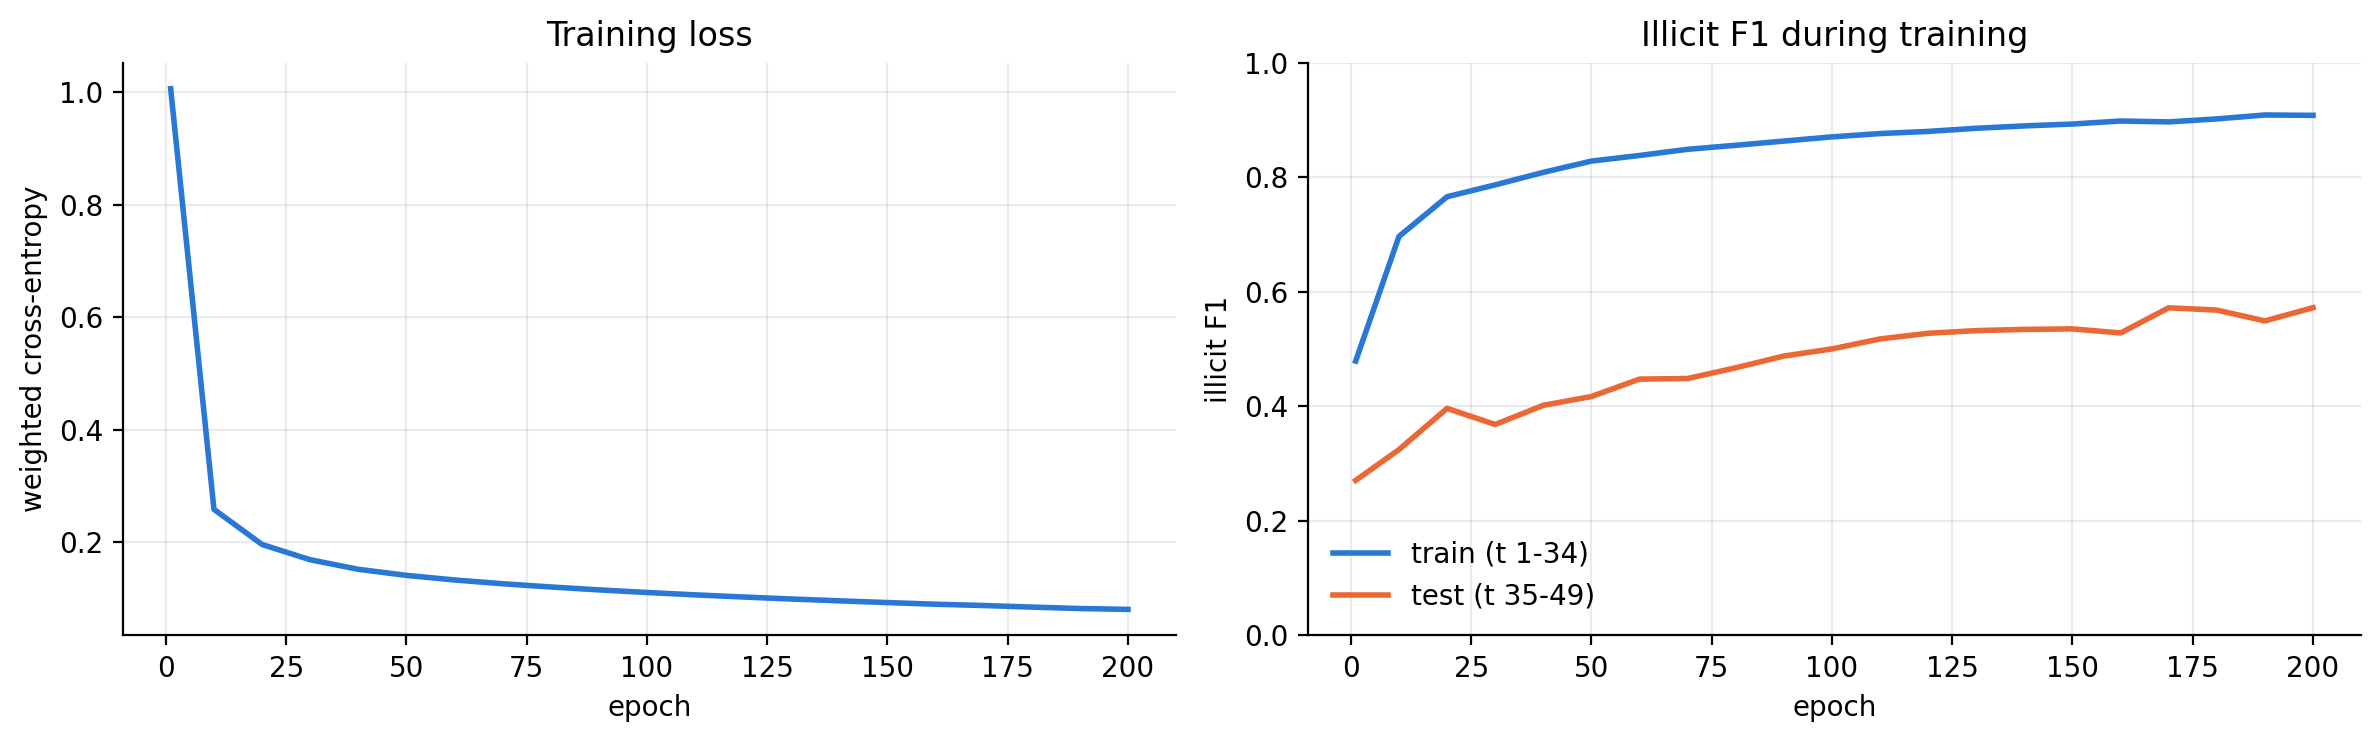
\includegraphics[width=\linewidth]{figures/training_curves.png}
  \caption{Training loss (left) and illicit F1 on the training and test periods (right). The test curve is plotted only; it
  is not used to choose the epoch.}
  \label{fig:curves}
\end{figure}

\begin{figure}[H]
  \centering
  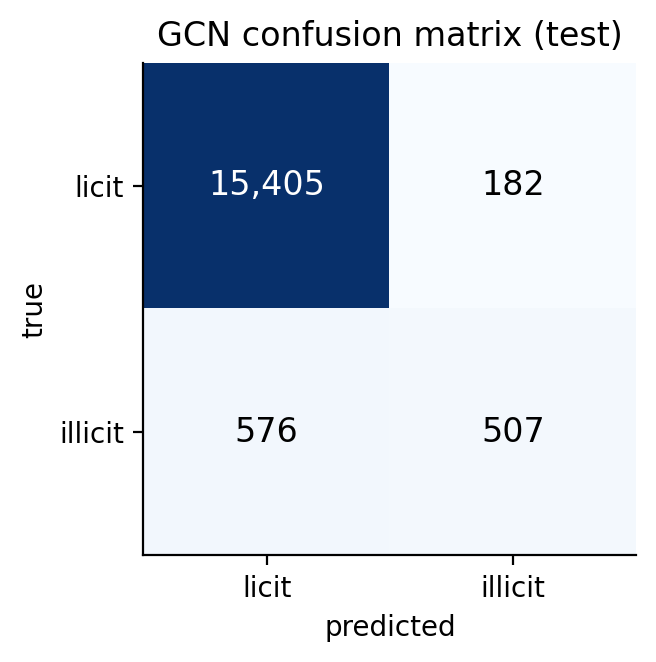
\includegraphics[width=0.36\linewidth]{figures/confusion_gcn.png}
  \caption{Confusion matrix of the GCN on the 16,670 labelled test transactions (threshold 0.5).}
  \label{fig:cm}
\end{figure}

\noindent After 200 epochs the GCN flags 689 transactions, of which 507 are illicit (precision 0.736), and it catches 507 of the
1,083 illicit ones (recall 0.468): illicit F1 = \textbf{0.572}, AP = 0.593, accuracy 95.5\%.

\subsection{Comparison with baselines (5 seeds)}
\begin{table}[H]
\centering\small
\begin{tabular}{llccccc}
\toprule
Features & Model & Precision & Recall & \textbf{Illicit F1} & AP & Weber et al.\ F1 \\
\midrule
AF (165) & Logistic Regression & 0.311 & 0.680 & 0.427 & 0.322 & 0.481 \\
         & MLP ($\Ahat = I$)   & 0.556 & 0.539 & 0.546 $\pm$ 0.009 & 0.443 & 0.653 \\
         & \textbf{GCN}        & 0.786 & 0.439 & 0.560 $\pm$ 0.034 & \textbf{0.604} & 0.628 \\
         & Skip-GCN            & 0.756 & 0.466 & 0.575 $\pm$ 0.024 & 0.597 & 0.705 \\
         & Random Forest       & 0.923 & 0.722 & \textbf{0.810 $\pm$ 0.004} & 0.783 & 0.788 \\
         & RF + GCN embedding  & 0.924 & 0.719 & 0.809 $\pm$ 0.010 & 0.777 & 0.796$^{*}$ \\
\midrule
LF (93)  & Logistic Regression & 0.393 & 0.714 & 0.507 & 0.299 & 0.457 \\
         & MLP ($\Ahat = I$)   & 0.447 & 0.745 & 0.559 $\pm$ 0.017 & 0.519 & 0.649 \\
         & \textbf{GCN}        & 0.428 & 0.599 & 0.495 $\pm$ 0.018 & \textbf{0.526} & -- \\
         & Skip-GCN            & 0.386 & 0.619 & 0.475 $\pm$ 0.014 & 0.493 & -- \\
         & Random Forest       & 0.848 & 0.705 & \textbf{0.770 $\pm$ 0.004} & 0.770 & 0.694 \\
\bottomrule
\end{tabular}
\caption{Test performance (time steps 35--49), mean over seeds 42, 1, 2, 3, 4 ($\pm$ std of the illicit F1; Logistic
Regression is deterministic). The last column gives the published illicit F1 of Weber et al.\ \cite{weber} for the same split.
$^{*}$Weber et al.\ used embeddings of a GCN trained with their settings (``AF+NE'').}
\label{tab:final}
\end{table}

\begin{figure}[H]
  \centering
  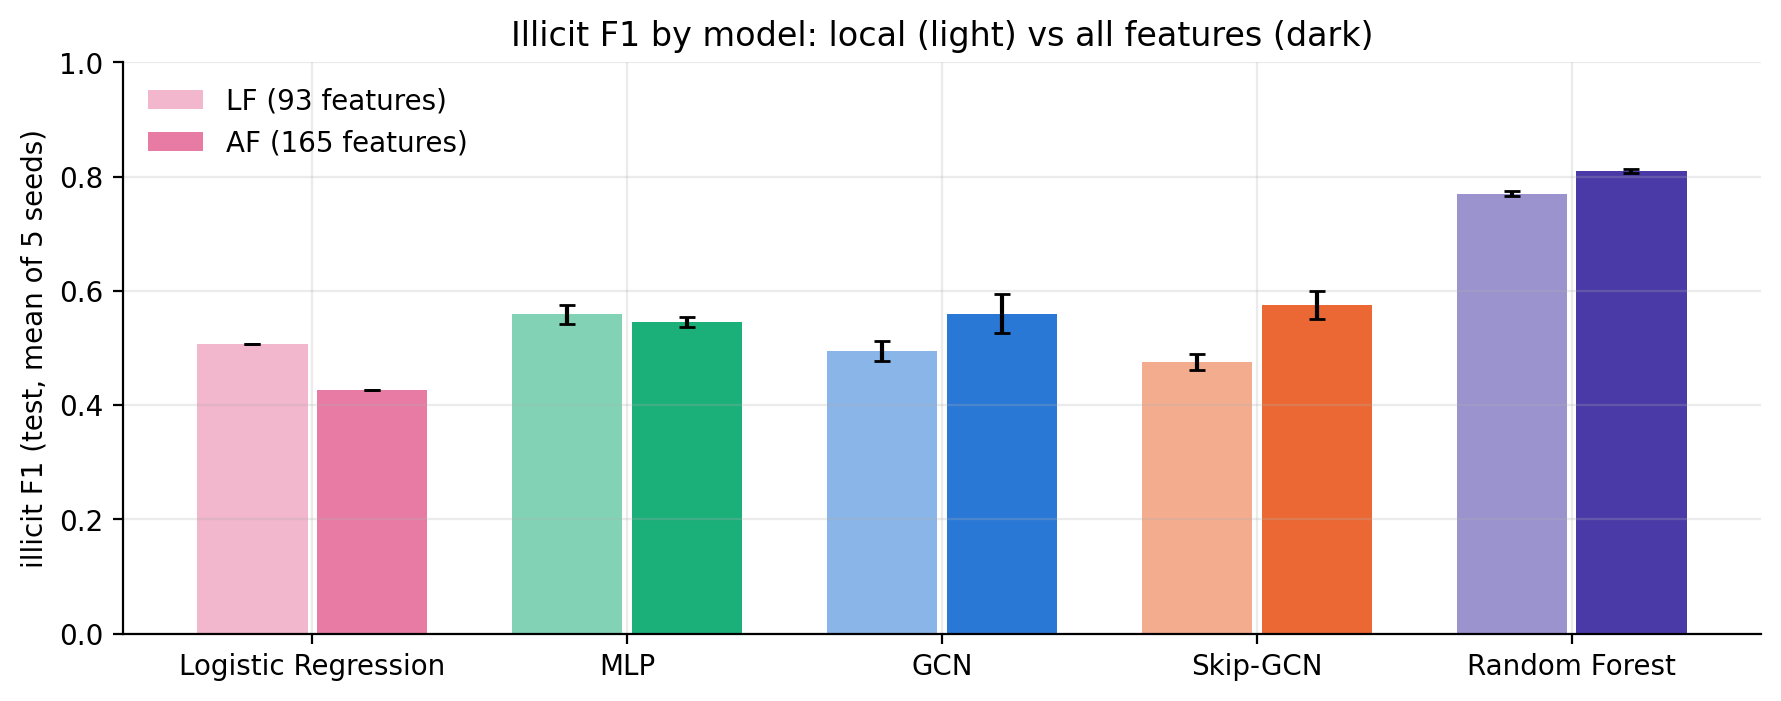
\includegraphics[width=0.85\linewidth]{figures/model_comparison.png}
  \caption{Illicit F1 of every model with local features (light) and all features (dark); error bars are one standard deviation over 5 seeds.}
  \label{fig:comparison}
\end{figure}

\subsection{Performance over time}
\begin{figure}[H]
  \centering
  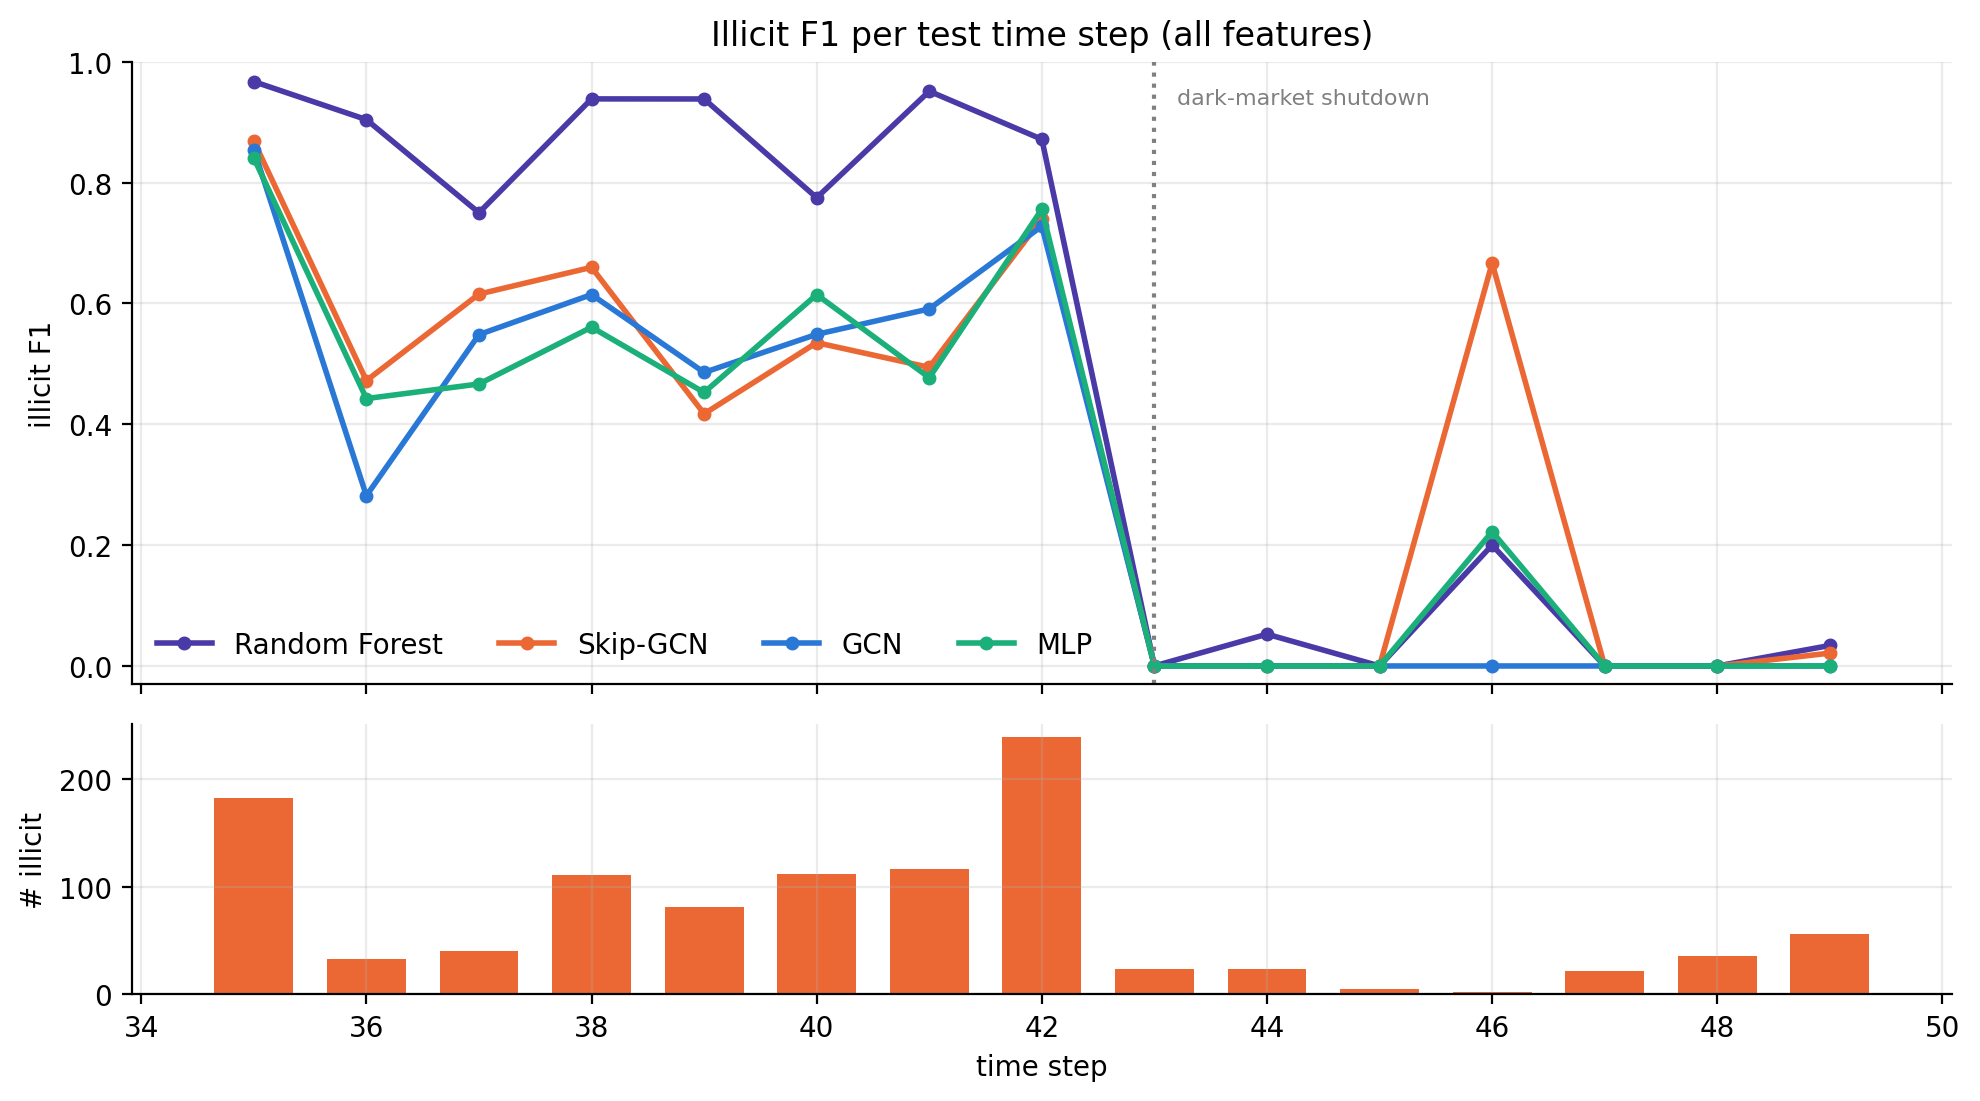
\includegraphics[width=0.9\linewidth]{figures/f1_per_timestep.png}
  \caption{Illicit F1 of each model per test time step (seed 42, all features), with the number of illicit transactions per step below.}
  \label{fig:perstep}
\end{figure}

\subsection{Depth and over-smoothing}
\begin{table}[H]
\centering\small
\begin{tabular}{lccccc}
\toprule
Layers & 1 & 2 & 3 & 4 & 6 \\
\midrule
Illicit F1 (test)          & 0.273 & \textbf{0.501} & 0.422 & 0.385 & 0.336 \\
std over 2 seeds           & 0.002 & 0.021 & 0.032 & 0.004 & 0.022 \\
Cosine sim.\ of last hidden layer & -- & 0.410 & 0.674 & 0.902 & 0.849 \\
\bottomrule
\end{tabular}
\caption{GCNs of increasing depth on local features (seeds 42 and 1). A 1-layer GCN has no hidden layer.}
\label{tab:depth}
\end{table}
\begin{figure}[H]
  \centering
  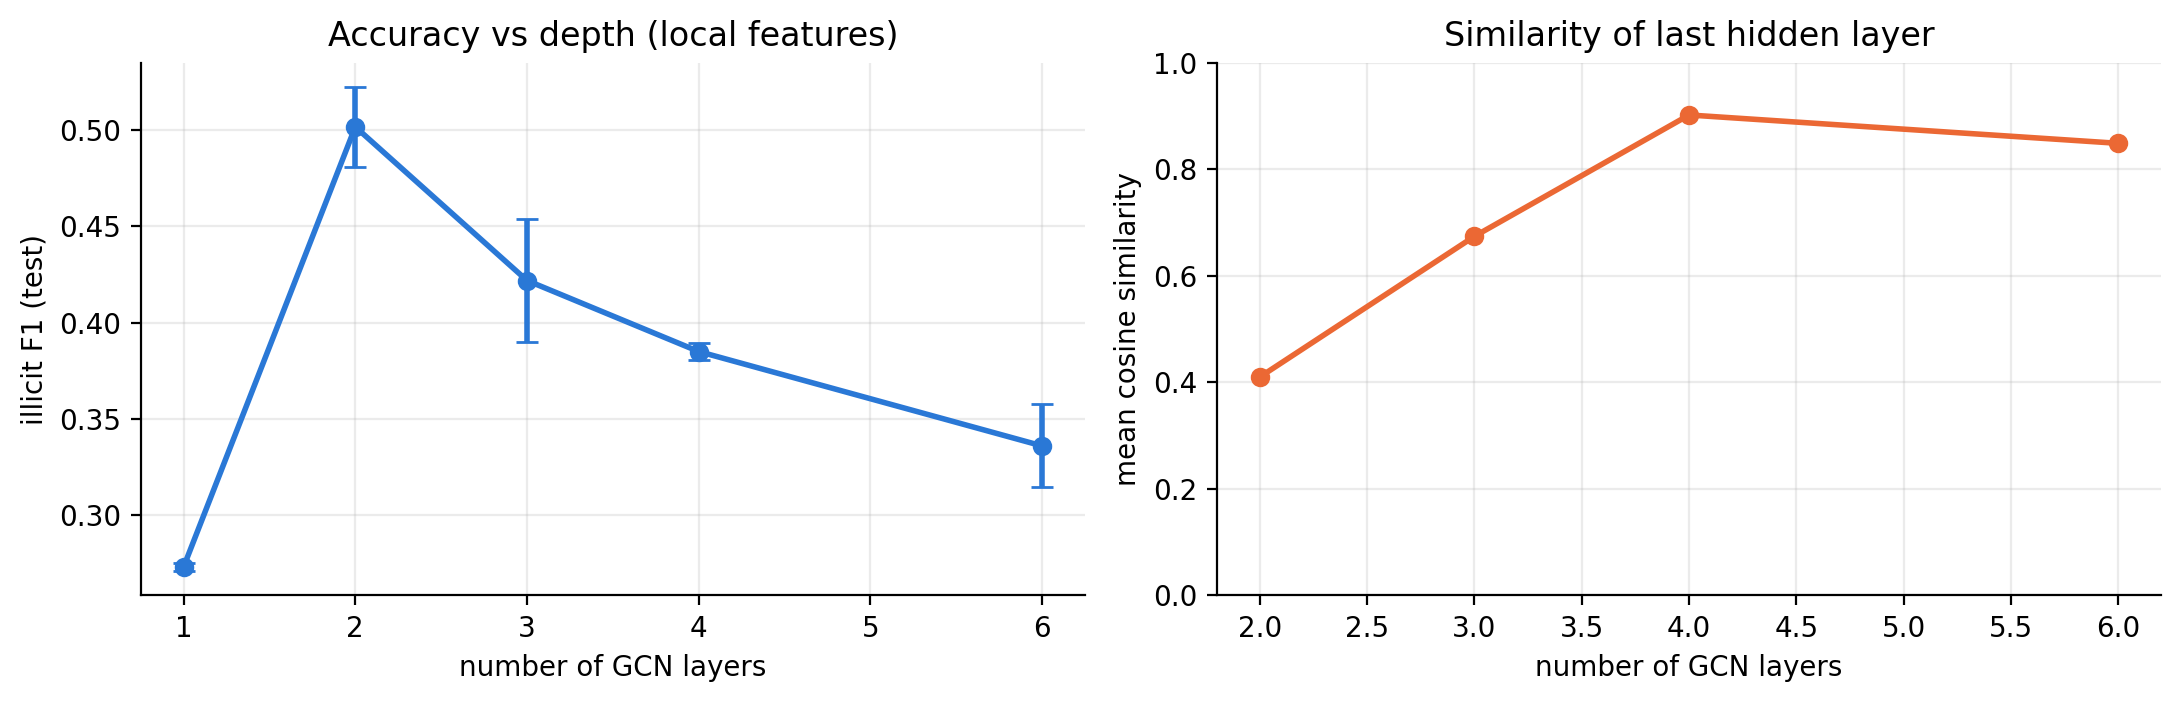
\includegraphics[width=0.9\linewidth]{figures/depth.png}
  \caption{Illicit F1 (left) and mean pairwise cosine similarity of the last hidden layer on 2,000 test transactions (right) versus depth.}
  \label{fig:depth}
\end{figure}

%=====================================================================
\section{Analysis and Limitations}
%=====================================================================
\subsection{Training behaviour}
The first loss is 1.007, above the $\ln 2 \approx 0.693$ of a uniform guess, because the randomly initialised network
starts out confidently wrong on some nodes; within 20 epochs it falls to 0.196 and then decreases smoothly to 0.081
(Fig.~\ref{fig:curves}). The curve has no dropout noise because we use none. Training illicit F1 climbs quickly to about 0.77 and
keeps improving slowly to 0.91, while the test F1 rises more gradually from 0.27 to 0.57 and is still increasing at epoch 200. We
did not extend training, because choosing the epoch from this curve would amount to tuning on the test set.

\subsection{Imbalance and the choice of metric}
Test accuracy is 95.5\%, only two points above the 93.5\% of a model that never flags anything. The illicit F1 of 0.572 is a
far more honest picture: the model misses more than half of the illicit transactions. The confusion matrix shows the character of the
GCN: when it flags a transaction it is usually right (precision 0.74; 0.79 on average over seeds), but it is conservative (recall
0.44--0.47). Even with the 0.3/0.7 class weights, the effective weight of the illicit class ($0.7\times3{,}462$) is still below that of
the licit class ($0.3\times26{,}432$), so the 0.5 threshold sits on the cautious side. A bank would move the threshold according to how
many alerts its investigators can handle; the threshold-free AP measures how well the model ranks transactions, independent of
that choice.

\subsection{What does the graph add?}
Comparing the GCN with the identical network that uses $\Ahat = I$ (the MLP) isolates the graph:
\begin{itemize}
  \item \textbf{With all features}, the graph makes the classifier much more precise: precision rises from 0.556 to 0.786 and AP from
        0.443 to 0.604 (+16 points), while recall drops from 0.539 to 0.439. At the fixed 0.5 threshold, illicit F1 improves only
        slightly (0.546 $\to$ 0.560, within one standard deviation). The Skip-GCN, which keeps a direct path for each transaction's own
        features, has the best F1 of the neural models (0.575).
  \item \textbf{With local features only}, the graph does \emph{not} improve F1 (0.559 for the MLP versus 0.495 for the GCN), and
        AP is about the same (0.519 versus 0.526).
\end{itemize}
The second result goes against the intuition that the graph should matter most when the hand-made neighbourhood features are removed.
It is consistent with the original study, where the MLP (0.653) also beat the GCN (0.628) on F1. We see three plausible reasons, which
we did not test separately.
(1) \emph{Mixing with unlabelled nodes}: 77\% of transactions are unlabelled, and an average degree of 2.3 means that
Eq.~(\ref{eq:node}) replaces roughly half to two thirds of a node's own signal with that of its neighbours, most of which carry no
supervision.
(2) \emph{Class-level rather than node-level homophily}: 95\% of labelled edges are same-class, but this figure is dominated by
licit--licit edges. A labelled neighbour of an illicit transaction is illicit only 54\% of the time, so averaging can dilute exactly
the rare signal we are looking for.
(3) \emph{Distribution shift}: test time steps are new graphs, and structural patterns learned on time steps 1--34 transfer less
well than per-transaction features (the GCN reaches a training F1 of 0.91 but a test F1 of 0.57).
The graph therefore helps a neural model \emph{rank} transactions, and it helps most when combined with features that already
describe the neighbourhood, but it is not a free improvement on this dataset.

\subsection{Comparison with the published results and the Random Forest}
Our Random Forest (0.810 with AF, 0.770 with LF) matches or exceeds Weber et al.\ (0.788, 0.694), and our GCN (0.560 $\pm$ 0.034) and
Skip-GCN (0.575) are below their 0.628 and 0.705. The gap is plausibly due to training: they trained for 1,000 epochs at learning rate
0.001, while we used the Kipf--Welling defaults for 200 epochs without tuning, and our test curve was still rising. The Random Forest is
clearly the strongest single model. Tree ensembles handle heavy-tailed, heterogeneous tabular features (counts, amounts, fees)
without scaling, and they model sharp thresholds and feature interactions that a 100-unit network smooths over. Adding the GCN's
hidden layer to the Random Forest's inputs did not help (0.809 versus 0.810), unlike the small gain (0.788 $\to$ 0.796) reported by
Weber et al.\ with their better-trained GCN.

\subsection{The dark-market shutdown}
Figure~\ref{fig:perstep} is perhaps the most important result. Up to time step 42 every model performs reasonably, and the
Random Forest is excellent (F1 0.75--0.97). From time step 43, when a large darknet market was shut down, \emph{every} model collapses to
an F1 near zero. The spike at $t=46$ is noise: that time step contains only 2 illicit transactions. The criminals' behaviour changed,
and models trained on the past no longer recognise it. No choice of architecture fixes this: it is \textbf{concept drift}, and in
practice it calls for continual retraining with fresh labels, drift monitoring, and models that detect \emph{anomalies} rather than
only known patterns. Temporal models such as EvolveGCN \cite{evolvegcn} were proposed for this reason, yet Weber et al.\ report that
they too fail after the shutdown.

\subsection{Over-smoothing}
\textbf{Why it happens.} $\Ahat$ is symmetric with eigenvalues in $(-1,1]$. On a connected component its largest eigenvalue is 1,
with eigenvector $\pi \propto \tilde D^{1/2}\mathbf 1$, and all other eigenvalues satisfy $|\mu_i|<1$ (self-loops rule out $-1$).
Therefore
\[
  \Ahat^{k}H = \pi\pi^\top H + \sum_{i\ge2}\mu_i^{k}\,u_iu_i^\top H \;\longrightarrow\; \pi\pi^\top H \qquad (k\to\infty),
\]
so every row becomes a multiple of the same vector: all transactions in a time step end up with the same representation direction
\cite{li,oono}. $\Ahat$ is a low-pass filter, and each layer removes a little more of the high-frequency information that distinguishes
a node from its neighbours.

\textbf{What we observe.} Table~\ref{tab:depth} shows this in trained models. A 1-layer GCN is linear and weak (0.273). Two layers are
best (0.501). Beyond that, F1 falls steadily (0.422, 0.385, 0.336) while the cosine similarity of the last hidden layer rises from 0.41
to 0.90 at four layers. The value at six layers (0.85) is slightly lower and varies more between seeds (0.09 std), which we attribute to
optimisation becoming unstable in a deep network without residual connections or normalisation. Because each Elliptic time step is its
own component of up to 7,880 nodes, deep GCNs push illicit and licit transactions of the same time step towards one representation,
which is exactly what a fraud detector must avoid. This is why GCNs are used with only two or three layers in practice.

\subsection{Limitations}
\textbf{Of our experiment}
\begin{itemize}
  \item Hyperparameters were fixed, not tuned. A validation period (e.g.\ time steps 30--34) could be used to tune the learning rate,
        epochs, class weights and decision threshold; our GCN is likely under-trained relative to Weber et al.
  \item Five seeds (two for the depth study) give rough standard deviations, and differences below about 2 F1 points between
        neural models are not significant.
  \item The test period contains only 1,083 illicit transactions, and the post-shutdown steps contain very few, so per-step F1
        values after $t=43$ are noisy.
  \item The 0.5 threshold is not optimal for F1 for any model; AP is reported to compensate.
\end{itemize}
\textbf{Of the vanilla GCN on this problem}
\begin{itemize}
  \item \emph{Fixed, isotropic aggregation}: every neighbour is weighted only by degree. Attention (GAT) or learned neighbour
        weighting could separate an illicit node's relevant links from its licit ones.
  \item \emph{Direction is ignored}: we symmetrise the graph, although money flow is directed; the in- and out-neighbourhoods of a
        laundering transaction mean different things.
  \item \emph{Static and transductive}: the model cannot adapt to drift and needs the whole graph in memory
        (remedies: GraphSAGE-style sampling, temporal GNNs, periodic retraining).
  \item \emph{Over-smoothing} limits depth (remedies: residual/skip connections, JK-Net, APPNP, DropEdge).
\end{itemize}

\subsection{Conclusion}
We implemented a two-layer GCN from scratch, as sparse matrix products $\Ahat(HW)$, and applied it to a real anti-money-laundering task
on 203,769 Bitcoin transactions. On future transactions it reaches an illicit F1 of 0.560 $\pm$ 0.034 (0.572 for seed 42). Compared with the
same network without the graph, it is far more precise (0.79 versus 0.56) and ranks illicit transactions much better (AP 0.60 versus 0.44).
The graph is not a free improvement, though: with local features only it does not beat the MLP, and a Random Forest on tabular
features remains the strongest model (0.810), as in the original benchmark. The per-time-step analysis shows the most important lesson of
the dataset: after a dark-market shutdown every model fails, so in real AML systems handling concept drift matters more than the choice
between a GCN and a tree ensemble. The depth study confirms over-smoothing in trained models and explains why GCNs are kept shallow.

\begin{thebibliography}{9}\small
\bibitem{kipf} T.~N.~Kipf and M.~Welling. Semi-Supervised Classification with Graph Convolutional Networks. \emph{ICLR}, 2017.
\bibitem{weber} M.~Weber, G.~Domeniconi, J.~Chen, D.~K.~I.~Weidele, C.~Bellei, T.~Robinson and C.~E.~Leiserson. Anti-Money Laundering in
Bitcoin: Experimenting with Graph Convolutional Networks for Financial Forensics. \emph{KDD Workshop on Anomaly Detection in Finance}, 2019.
\bibitem{evolvegcn} A.~Pareja, G.~Domeniconi, J.~Chen, T.~Ma, T.~Suzumura, H.~Kanezashi, T.~Kaler, T.~B.~Schardl and C.~E.~Leiserson.
EvolveGCN: Evolving Graph Convolutional Networks for Dynamic Graphs. \emph{AAAI}, 2020.
\bibitem{li} Q.~Li, Z.~Han and X.-M.~Wu. Deeper Insights into Graph Convolutional Networks for Semi-Supervised Learning. \emph{AAAI}, 2018.
\bibitem{oono} K.~Oono and T.~Suzuki. Graph Neural Networks Exponentially Lose Expressive Power for Node Classification. \emph{ICLR}, 2020.
\bibitem{pyg} M.~Fey and J.~E.~Lenssen. Fast Graph Representation Learning with PyTorch Geometric. \emph{ICLR Workshop}, 2019.
\end{thebibliography}
\end{document}
